\label{cap:caracterizacion}
\Needspace{.16\textheight}\section{Propósito y alcance de la auditoría}
Antes de construir un modelo es necesario entender qué contiene cada archivo y cómo puede utilizarse. Por esta razón, se revisaron las siete tablas de OULAD, sus relaciones y sus fechas. Este trabajo corresponde al primer objetivo específico y a la comprensión de datos de CRISP-DM. Los resultados corresponden a la revisión documentada de las fuentes disponibles.

Los archivos, las fechas de ejecución y las comprobaciones realizadas se describen en el Anexo~\ref{anexo:reproducibilidad}.

OULAD reúne información de matrícula, evaluaciones e interacciones con recursos virtuales \cite{sdata2017171}. La revisión examinó los archivos disponibles en el proyecto. Se utilizaron huellas SHA-256, códigos que permiten detectar si un archivo cambió, para comprobar que las fuentes se conservaron durante el procesamiento. Estas huellas identifican los archivos utilizados, pero no certifican su procedencia.

\Needspace{.16\textheight}\section{Estructura y unidad de análisis}
La Tabla~\ref{rev01:dimensiones} permite distinguir el tamaño de las fuentes de la cantidad de unidades analizadas. Las filas de interacciones y entregas describen registros asociados a una inscripción; no representan personas adicionales.
Se verificaron 32\,593 inscripciones correspondientes a 28\,785 personas, 7 módulos y 22 combinaciones de módulo y presentación. La inscripción se identifica mediante la clave compuesta de estudiante, módulo y presentación. Se encontraron 3\,538 personas con más de una inscripción; por ello, el tamaño de la tabla no debe presentarse como número de estudiantes distintos.

\Needspace{0.23\textheight}\begingroup\small\setlength{\tabcolsep}{3pt}\renewcommand{\arraystretch}{1.16}
\begin{longtable}{>{\raggedright\arraybackslash}p{0.56\linewidth}>{\raggedright\arraybackslash}p{0.23\linewidth}>{\raggedright\arraybackslash}p{0.15\linewidth}}
\caption{Dimensiones verificadas de las fuentes locales.}\label{rev01:dimensiones}\\
\toprule
\textbf{Tabla} & \textbf{Filas} & \textbf{Columnas} \\
\midrule\endfirsthead
\toprule
\textbf{Tabla} & \textbf{Filas} & \textbf{Columnas} \\
\midrule\endhead
\bottomrule\endfoot
courses & 22 & 3 \\*
assessments & 206 & 6 \\*
vle & 6\,364 & 6 \\*
studentInfo & 32\,593 & 12 \\*
studentRegistration & 32\,593 & 5 \\*
studentAssessment & 173\,912 & 5 \\*
studentVle & 10\,655\,280 & 6 \\*
\end{longtable}\endgroup
Para reunir la información, se utilizaron los identificadores de estudiante, módulo y presentación, junto con los de evaluación o recurso cuando correspondía. Por ejemplo, una persona puede estar inscrita en dos módulos: sus entregas y clics deben asociarse a la inscripción correspondiente, sin mezclar ambos cursos. Un módulo identifica el curso y una presentación identifica una edición concreta de ese curso. Se comprobó que cada evaluación y cada recurso correspondieran a la inscripción, el módulo y la presentación esperados. Las nueve verificaciones de relaciones no encontraron registros sin correspondencia. Las uniones de información y matrícula conservaron una fila por inscripción; el calendario se vinculó con la presentación correspondiente.

\Needspace{.16\textheight}\section{Registros repetidos y sensibilidad del volumen}
Las tablas de estudiantes, matrículas, cursos y entregas no presentaron claves repetidas. En cambio, el registro de actividad VLE contiene filas idénticas y filas que comparten estudiante, módulo, presentación, recurso y día. Una fila idéntica repite todos los campos; una repetición de clave comparte esos identificadores, aunque otro campo, como el número de clics, pueda ser distinto. La tabla cuenta las filas adicionales después de conservar una primera aparición de cada combinación. Los archivos no incluyen un identificador de sesión que permita explicar esas repeticiones. Por ello, no se interpretan como sesiones diferentes.
\Needspace{0.23\textheight}\begingroup\small\setlength{\tabcolsep}{3pt}\renewcommand{\arraystretch}{1.16}
\begin{longtable}{>{\raggedright\arraybackslash}p{0.46\linewidth}>{\raggedright\arraybackslash}p{0.23\linewidth}>{\raggedright\arraybackslash}p{0.25\linewidth}}
\caption{Filas adicionales a la primera ocurrencia de cada combinación.}\label{rev01:duplicados}\\
\toprule
\textbf{Tabla} & \textbf{Duplicados exactos} & \textbf{Repetidos de clave} \\
\midrule\endfirsthead
\toprule
\textbf{Tabla} & \textbf{Duplicados exactos} & \textbf{Repetidos de clave} \\
\midrule\endhead
\bottomrule\endfoot
courses & 0 & 0 \\*
assessments & 0 & 0 \\*
vle & 0 & 0 \\*
studentInfo & 0 & 0 \\*
studentRegistration & 0 & 0 \\*
studentAssessment & 0 & 0 \\*
studentVle & 787\,170 & 2\,195\,960 \\*
\end{longtable}\endgroup
Para construir los indicadores se conservan las filas originales. Esta decisión mantiene la información recibida, porque los archivos no permiten distinguir cuáles repeticiones serían errores y cuáles podrían corresponder a actividad válida. Se reconoce que conservarlas puede aumentar los conteos si existen duplicados de captura. Para examinar cuánto cambia el resultado, se realiza una segunda comparación retirando únicamente las filas idénticas. La Tabla~\ref{multi01:sensibilidad} presenta la alternativa de retirar repeticiones exactas dentro de cada ventana inclusiva de días 0 a $t$. Los totales corresponden a toda la actividad registrada en esas fechas, antes de restringirla a la población elegible; por ello, no equivalen a los totales de los conjuntos analíticos. La reducción se sitúa aproximadamente entre 3,27 y 3,50 por ciento. Esta comparación permite observar cuánto cambia el total de clics al retirar filas idénticas. No permite establecer si esas filas representan errores o interacciones válidas; tampoco evalúa cómo cambiarían las predicciones de un modelo.

\Needspace{0.3\textheight}
\Needspace{0.23\textheight}\begingroup\small\setlength{\tabcolsep}{3pt}\renewcommand{\arraystretch}{1.16}
\begin{longtable}{>{\raggedright\arraybackslash}p{0.12\linewidth}>{\raggedright\arraybackslash}p{0.28\linewidth}>{\raggedright\arraybackslash}p{0.28\linewidth}>{\raggedright\arraybackslash}p{0.23\linewidth}}
\caption{Sensibilidad de los clics en cada ventana, sobre la fuente completa.}\label{multi01:sensibilidad}\\
\toprule
\textbf{Corte} & \textbf{Clics originales} & \textbf{Sin duplicados} & \textbf{Reducción (\%)} \\
\midrule\endfirsthead
\toprule
\textbf{Corte} & \textbf{Clics originales} & \textbf{Sin duplicados} & \textbf{Reducción (\%)} \\
\midrule\endhead
\bottomrule\endfoot
7 & 2\,218\,326 & 2\,140\,648 & 3,50 \\*
14 & 4\,047\,355 & 3\,906\,767 & 3,47 \\*
28 & 7\,945\,783 & 7\,685\,825 & 3,27 \\*
42 & 10\,656\,511 & 10\,303\,183 & 3,32 \\*
56 & 13\,256\,804 & 12\,815\,335 & 3,33 \\*
\end{longtable}\endgroup

\Needspace{.16\textheight}\section{Información faltante y revisión de valores y fechas}
Antes de construir los indicadores, se revisó qué información estaba disponible y si los valores registrados eran coherentes con la descripción de los datos. Esta revisión permitió identificar campos vacíos, comprobar los valores de las evaluaciones y examinar las fechas de matrícula, entrega y retiro. Cada situación requiere una interpretación distinta, pues un campo vacío no siempre representa el mismo problema.

Por ejemplo, una inscripción sin fecha de retiro se trata en este estudio como un caso sin retiro registrado. Esto no permite afirmar, por sí solo, que el estudiante haya aprobado el curso. En cambio, cuando falta la fecha de matrícula, no se puede comprobar si la inscripción ya existía en el momento elegido para hacer la predicción. A ese momento se le denomina día de corte. Si se quisiera predecir al finalizar el día 28, sería necesario saber si la matrícula ocurrió a más tardar ese día.

Algo similar sucede con las evaluaciones. Puede existir un registro de entrega sin que aparezca su calificación; por ello, la ausencia de una nota no debe interpretarse automáticamente como una actividad no entregada. La Tabla~\ref{rev01:faltantes} presenta los campos con información faltante. En cada caso, el porcentaje se calcula sobre el total de filas del archivo correspondiente, no sobre una misma cantidad de estudiantes.

\begingroup\small\setlength{\tabcolsep}{3pt}\renewcommand{\arraystretch}{1.16}
\Needspace{.42\textheight}\begin{longtable}{p{.21\linewidth}p{.35\linewidth}r r r}
\caption{Información faltante en los archivos revisados.}\label{rev01:faltantes}\\
\toprule
Archivo & Campo sin información & Ausentes & Total & \% \\
\midrule\endfirsthead
Archivo & Campo sin información & Ausentes & Total & \% \\
\midrule\endhead
\bottomrule\endfoot
assessments & Fecha de la evaluación & 11 & 206 & 5,34 \\
vle & Semana prevista de inicio de uso del recurso & 5\,243 & 6\,364 & 82,39 \\
vle & Semana prevista de finalización de uso del recurso & 5\,243 & 6\,364 & 82,39 \\
studentInfo & Categoría del índice de privación múltiple del área de residencia (IMD) & 1\,111 & 32\,593 & 3,41 \\
studentRegistration & Fecha de matrícula & 45 & 32\,593 & 0,14 \\
studentRegistration & Fecha de retiro & 22\,521 & 32\,593 & 69,10 \\
studentAssessment & Calificación de la evaluación & 173 & 173\,912 & 0,10 \\
\end{longtable}\endgroup

La ausencia de fechas de retiro debe leerse de acuerdo con la definición anterior y no como una pérdida general de información. Asimismo, las semanas previstas de uso de los recursos describen su programación; su ausencia no significa que no existan registros de interacción con esos materiales. El índice de privación múltiple (IMD, \textit{Index of Multiple Deprivation}) corresponde al área de residencia, por lo que no constituye una medida directa de los ingresos personales del estudiante.

También se revisaron las calificaciones y los conteos de clics. Los resultados guardados de la revisión no registran calificaciones fuera del intervalo de 0 a 100 ni conteos de clics menores o iguales a cero en las filas del archivo de interacciones. Esta última comprobación se refiere a los registros existentes: no significa que todos los estudiantes hayan tenido actividad todos los días.

OULAD incluye además el campo \texttt{is\_banked}, que indica si el resultado de una evaluación fue trasladado desde una edición anterior del curso. En la revisión se comprobó que este campo solo contuviera los valores 0 y 1; no se encontraron valores distintos. Esta distinción importa porque un resultado reconocido de una edición anterior no equivale a una nueva entrega durante el periodo que se está observando \cite{sdata2017171}.

Otra comprobación examinó el peso de las evaluaciones, es decir, el porcentaje asignado a cada una. Las actividades realizadas durante el curso y los exámenes se revisaron por separado, de acuerdo con la organización descrita en OULAD. Por ello, sumar todos sus pesos y exigir que el total sea siempre 200 no se utilizó como regla general para identificar errores. La tabla detallada de esta comprobación se conserva entre las salidas del análisis \cite{sdata2017171}.

Las fechas también necesitan una lectura particular. En OULAD, el día 0 corresponde al inicio de la edición del curso y los números negativos indican momentos anteriores. Por ejemplo, una matrícula registrada en el día $-10$ ocurrió diez días antes del inicio. Por esta razón, las fechas negativas no se eliminaron automáticamente. La Tabla~\ref{rev01:fechas} reúne los casos identificados al revisar las fechas y los resultados reconocidos de otras ediciones.

\begingroup\small\setlength{\tabcolsep}{3pt}\renewcommand{\arraystretch}{1.16}
\begin{longtable}{p{.78\linewidth}r}
\caption{Casos identificados en la revisión de fechas y evaluaciones.}\label{rev01:fechas}\\
\toprule
Situación & Número de casos \\
\midrule\endfirsthead
Situación & Número de casos \\
\midrule\endhead
\bottomrule\endfoot
Inscripciones sin fecha de matrícula & 45 \\
Inscripciones con matrícula posterior al día 28 & 16 \\
Inscripciones con retiro posterior al final de la edición del curso & 1 \\
Registros de entrega anteriores al inicio del curso & 2\,057 \\
Resultados de evaluaciones reconocidos de una edición anterior & 1\,909 \\
Registros de interacción anteriores a la matrícula & 0 \\
Registros de interacción posteriores al retiro & 29\,440 \\
Registros de entrega posteriores al retiro & 601 \\
\end{longtable}\endgroup

El día 28 se utiliza en esta tabla como referencia para describir las fechas de matrícula. La selección de inscripciones para cada día de predicción se realiza por separado en el capítulo siguiente. Además, los casos de la tabla corresponden a distintos tipos de registro y pueden coincidir entre sí; no deben sumarse como si fueran estudiantes diferentes.

Se identificaron interacciones y entregas con fecha posterior al retiro. Los archivos disponibles no permiten establecer por qué ocurrió esta situación. Sin embargo, esos registros no pueden emplearse como información previa para anticipar un retiro que ya había sucedido. Por ejemplo, si una inscripción tiene un retiro registrado en el día 20, una interacción del día 25 no sirve para predecir anticipadamente ese retiro.

Finalmente, identificar información faltante permite conocer una limitación de los datos, pero no explica por qué falta. La revisión no permite determinar si esas ausencias se relacionan con características observadas de los estudiantes o con información que no está disponible. Esta limitación debe considerarse al interpretar los análisis posteriores.

\Needspace{.16\textheight}\section{Definición administrativa del retiro}
En esta descripción, un retiro administrativo es una inscripción que tiene una fecha registrada en el campo \texttt{date\_unregistration}. La fecha permite ubicar la salida respecto al inicio del curso, pero no establece su motivo. El retiro futuro añade una condición: debe ocurrir después del día en que se haría la predicción y hasta el final de esa edición del curso.

La Tabla~\ref{rev01:retiro} organiza las fechas de toda la fuente usando el día 28 como referencia descriptiva. Esta elección no significa que solo se estudie ese día. En el Capítulo~\ref{cap:ingenieria} se determina por separado quiénes pueden incluirse en los cortes 7, 14, 28, 42 y 56. La Figura~\ref{editorial:cascada28} muestra, paso a paso, cuántas inscripciones permanecen después de aplicar cada condición en el corte 28.

La presencia de fecha de retiro se observó en 10\,072 de 32\,593 inscripciones (30,90\,\%). Esta proporción describe la fuente completa. Incluye eventos anteriores al inicio y al corte de predicción, por lo que no es la prevalencia del retiro futuro.

\Needspace{0.23\textheight}\begingroup\small\setlength{\tabcolsep}{3pt}\renewcommand{\arraystretch}{1.16}
\begin{longtable}{>{\raggedright\arraybackslash}p{0.48\linewidth}>{\raggedright\arraybackslash}p{0.22\linewidth}>{\raggedright\arraybackslash}p{0.24\linewidth}}
\caption{Distribución administrativa del retiro.}\label{rev01:retiro}\\
\toprule
\textbf{Momento} & \textbf{Inscripciones} & \textbf{Porcentaje de la fuente} \\
\midrule\endfirsthead
\toprule
\textbf{Momento} & \textbf{Inscripciones} & \textbf{Porcentaje de la fuente} \\
\midrule\endhead
\bottomrule\endfoot
Antes del inicio & 2\,678 & 8,22 \\*
Después del día 28 & 5\,017 & 15,39 \\*
Día 28 & 15 & 0,05 \\*
Días 0 a 27 & 2\,362 & 7,25 \\*
Sin fecha de retiro & 22\,521 & 69,10 \\*
\end{longtable}\endgroup
\Needspace{0.18\textheight}\begingroup\small\setlength{\tabcolsep}{3pt}\renewcommand{\arraystretch}{1.16}
\begin{longtable}{>{\raggedright\arraybackslash}p{0.2106382978723404\linewidth}>{\raggedright\arraybackslash}p{0.17234042553191486\linewidth}>{\raggedright\arraybackslash}p{0.1627659574468085\linewidth}>{\raggedright\arraybackslash}p{0.1627659574468085\linewidth}>{\raggedright\arraybackslash}p{0.19148936170212766\linewidth}}
\caption{Contraste de fecha de retiro y resultado final; 0 = no, 1 = sí.}\label{rev01:discordancia}\\
\toprule
\textbf{Fecha presente} & \textbf{Distinction} & \textbf{Fail} & \textbf{Pass} & \textbf{Withdrawn} \\
\midrule\endfirsthead
\toprule
\textbf{Fecha presente} & \textbf{Distinction} & \textbf{Fail} & \textbf{Pass} & \textbf{Withdrawn} \\
\midrule\endhead
\bottomrule\endfoot
0 & 3\,024 & 7\,043 & 12\,361 & 93 \\*
1 & 0 & 9 & 0 & 10\,063 \\*
\end{longtable}\endgroup
Se identificaron 102 discordancias: 93 inscripciones con resultado Withdrawn carecen de fecha de retiro y nueve con fecha de retiro tienen resultado Fail. Estas diferencias se exportaron para revisión. Withdrawn identifica un resultado final de retiro y Fail un resultado de reprobación. Para este estudio se conserva la definición basada en la fecha administrativa, que permite ubicar cuándo ocurrió el retiro. Las diferencias entre campos se documentan y no permiten establecer si el retiro fue voluntario.

\begin{figure}[htbp]\centering
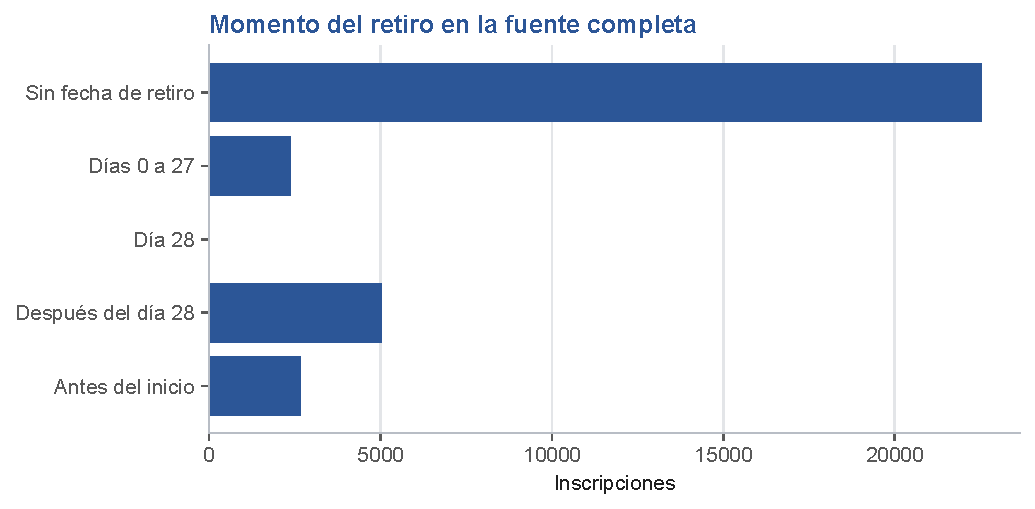
\includegraphics[width=.94\linewidth]{figuras_multiventana/01_momento_retiro.pdf}
\caption{Conteos de la fuente completa. El día 28 se mantiene separado de los eventos futuros.}\label{rev01:figretiro}\end{figure}
\Needspace{.16\textheight}\section{Balance de la auditoría y productos}
La revisión permitió relacionar las tablas mediante sus identificadores sin encontrar registros sin correspondencia en las comprobaciones realizadas. También identificó situaciones que requieren cuidado: filas repetidas, diferencias entre la fecha de retiro y el resultado final, y evaluaciones cuya calificación no puede situarse con certeza antes de la predicción.

Como resultado se prepararon tres archivos: una base que reúne la información de cada inscripción, un registro que suma los clics de cada inscripción por día y un archivo de entregas que incorpora los datos de la evaluación correspondiente. Estos productos permiten construir los indicadores del capítulo siguiente. No constituyen todavía un modelo de predicción.

Las tablas de revisión presentan los conteos de faltantes, repeticiones, fechas y relaciones entre archivos. El Anexo~\ref{anexo:reproducibilidad} identifica las salidas necesarias para consultar cada comprobación, junto con los registros de ejecución.

\Needspace{.16\textheight}\section{Distribución temporal del retiro}
La Figura~\ref{corr:histograma} muestra cuándo se registraron los retiros de las 10\,072 inscripciones con fecha disponible. El eje horizontal expresa días respecto al inicio del curso y la altura de cada barra cuenta los retiros en ese intervalo. Los valores negativos corresponden a salidas anteriores al inicio. Las líneas verticales ubican el inicio y los cinco días de corte, para distinguir lo que ya había ocurrido de lo que aún podría anticiparse.

Entre esos casos hay 2\,678 retiros anteriores al inicio. Se incluyen para describir la fuente, pero no son retiros futuros de los cortes estudiados. Por ello, los conteos de esta figura no deben compararse directamente con porcentajes calculados después de seleccionar las inscripciones de cada corte.

\begin{figure}[htbp]\centering
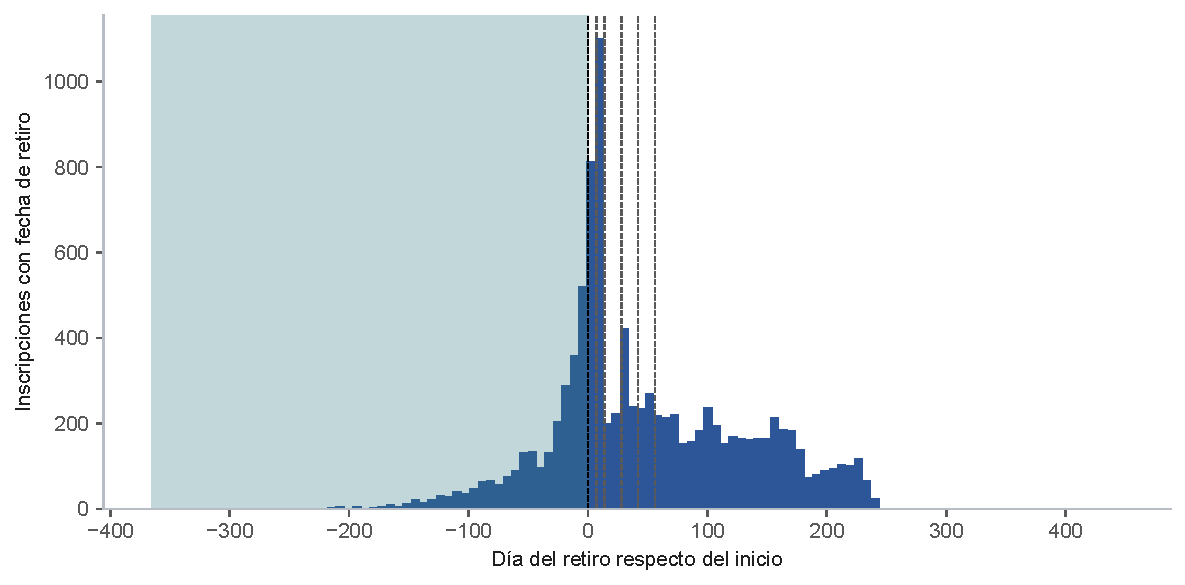
\includegraphics[width=.94\linewidth]{figuras_multiventana/01_fechas_retiro.pdf}
\caption{Distribución de fechas de retiro; líneas en el inicio y en los cortes 7, 14, 28, 42 y 56.}\label{corr:histograma}\end{figure}

\Needspace{.16\textheight}\section{Exploración estadística por corte}
\paragraph{Claves para leer los resultados}\label{lectura:contexto-cortes}
Las comparaciones siguientes utilizan como unidad una inscripción: la participación de una persona en un módulo y en una edición de ese módulo, denominada presentación. Una persona puede aportar varias inscripciones. El día de corte es el momento hasta el cual se reúne información, contado desde el inicio del curso. Se analizan los días 7, 14, 28, 42 y 56. En cada corte se incluyen las inscripciones cuya fecha de matrícula se conoce, que ya estaban matriculadas, que no se habían retirado hasta ese día y cuyo curso continúa después del corte.

El retiro futuro es el retiro registrado después del corte y hasta el final de la edición del curso. Por ejemplo, al analizar el día 28 se observa la actividad desde el día 0 hasta el 28, ambos incluidos. Una inscripción retirada el día 20 o el propio día 28 queda excluida; una retirada el día 40 puede incluirse y presentar retiro futuro, siempre que cumpla las demás condiciones y ese retiro ocurra antes de finalizar el curso o en su último día. La inactividad por sí sola no se considera retiro.

Los indicadores resumen aspectos de la participación: los clics acumulados expresan volumen; la proporción de días activos indica en qué parte de los días observados hubo actividad; y la recencia mide cuánto tiempo ha pasado desde la última interacción. El coeficiente de variación (CV) describe la variabilidad de los clics respecto de su promedio: su versión de calendario incluye los días sin clics y su versión activa considera solo los días con actividad. La tendencia compara periodos recientes, mientras las entregas describen la participación en las evaluaciones. Sus reglas y fórmulas se desarrollan en el capítulo~\ref{cap:ingenieria}.

Cada porcentaje de retiro utiliza como denominador las inscripciones elegibles del corte o de la categoría indicada. Al cambiar el corte cambian tanto el grupo incluido como el tiempo restante para observar un retiro; por ello, comparar esos porcentajes no equivale a seguir al mismo grupo durante todo el curso.

\Needspace{.14\textheight}\subsection{Propósito y alcance estadístico}
El análisis examina la distribución y las asociaciones de los indicadores construidos en los cortes 7, 14, 28, 42 y 56. Corresponde a una exploración previa al modelado: se analizan todos los datos elegibles y no se atribuyen a estos resultados propiedades de validación predictiva. Cada corte mantiene su propia población en riesgo y su evento futuro hasta el final de la presentación.

La exploración describe cómo se distribuyen los valores, cuánto varían y cuántos datos faltan. Se distingue entre un cero y un indicador que no puede calcularse: por ejemplo, no hay recencia cuando no existe actividad previa, ni proporción entregada cuando no hay evaluaciones programadas. Para localizar valores poco habituales se emplearon dos referencias. El rango intercuartílico mide la amplitud de la mitad central de los valores; la desviación absoluta mediana resume cuánto se alejan los valores de la mediana, que es el punto central de los datos ordenados. Ambas permiten señalar valores alejados del resto, pero no se utilizaron para eliminar registros. Estas medidas comparan cada valor con la dispersión habitual de los datos. Si la dispersión utilizada como referencia es cero, no se calcula el diagnóstico que requiere dividir por ella. Los valores señalados se conservan porque una actividad poco frecuente puede ser real; identificarla no demuestra que sea un error. Tampoco se deducen las causas de los datos faltantes a partir de su cantidad.

\Needspace{.14\textheight}\subsection{Asociaciones e incertidumbre dentro de cada corte}
La pregunta de esta comparación es si los valores observados de cada indicador difieren entre inscripciones con y sin retiro futuro. La Tabla~\ref{multi03:efectos} resume la dirección y magnitud de esas asociaciones; la Figura~\ref{multi03:figefectos} añade intervalos para una selección de indicadores. Su lectura conjunta distingue una estimación puntual de su incertidumbre.
Para resumir la comparación se utiliza el efecto biserial por rangos. Esta medida ordena los valores de ambos grupos y describe en cuál tienden a ser mayores; toma valores entre $-1$ y $1$. Se calcula a partir del estadístico de Mann--Whitney, contando también los valores iguales entre grupos \cite{revscipy}:
\[
r_{rb}=\frac{2U_1}{n_1n_0}-1.
\]
El grupo 1 reúne las inscripciones con retiro futuro y el grupo 0 las que no tienen ese evento registrado en el periodo de seguimiento. Los símbolos $n_1$ y $n_0$ indican cuántas inscripciones con datos disponibles hay en cada grupo. $U_1$ cuenta las comparaciones en las que el valor del grupo 1 supera al del grupo 0 y añade media unidad por cada empate. Así, $n_1n_0$ es el número total de pares que pueden compararse.

Por ejemplo, si los valores hipotéticos del grupo 1 fueran 2 y 4 clics, y los del grupo 0 fueran 3 y 5, solo uno de los cuatro pares tendría un valor mayor en el grupo 1. Se obtendría $U_1=1$ y $r_{rb}=2(1)/4-1=-0{,}5$. El signo negativo resume que, en este ejemplo, las inscripciones con retiro tienden a registrar menos clics. No expresa una disminución del 50\,\% en la probabilidad de retiro.

 Un efecto negativo indica valores generalmente menores en ese grupo y un efecto positivo indica valores mayores. Para cada indicador se utilizan las inscripciones de ambos grupos en las que ese indicador puede calcularse. Por ejemplo, la recencia requiere una interacción previa; las inscripciones sin actividad no entran en esa comparación, aunque sí puedan entrar al comparar el total de clics. Por ello, la cantidad de casos puede variar entre indicadores dentro de un mismo corte. Las estimaciones no son efectos causales ni medidas del rendimiento de un clasificador.

Para acompañar las asociaciones con una medida de incertidumbre, se construyeron intervalos del 95 por ciento mediante 5\,000 remuestreos. En cada repetición se seleccionaron personas con reposición y se conservaron juntas sus inscripciones, usando la semilla 20260908 \cite{revfield2007}. Seleccionar con reposición significa que una persona puede aparecer varias veces en una repetición y no aparecer en otra. Si tiene dos inscripciones, ambas se incluyen juntas cada vez que se selecciona a esa persona. Se recalcula la asociación en cada repetición y se toman los percentiles 2,5 y 97,5 de los resultados válidos como límites del intervalo. Así se reconoce que varias inscripciones de una misma persona pueden estar relacionadas. Los cursos observados se mantuvieron fijos; no se estimó la incertidumbre que surgiría al estudiar otros cursos. Un intervalo más amplio indica que la asociación estimada cambia más entre los remuestreos. El intervalo describe la incertidumbre de la asociación, no el rango de riesgo de un estudiante. Los intervalos corresponden a cada estimación por separado y son exploratorios: su solapamiento no se usa como prueba de diferencia entre ventanas.

\Needspace{.16\textheight}
\begingroup\small\setlength{\tabcolsep}{3pt}\renewcommand{\arraystretch}{1.16}
\begin{longtable}{>{\raggedright\arraybackslash}p{0.3375\linewidth}>{\raggedright\arraybackslash}p{0.1125\linewidth}>{\raggedright\arraybackslash}p{0.1125\linewidth}>{\raggedright\arraybackslash}p{0.1125\linewidth}>{\raggedright\arraybackslash}p{0.1125\linewidth}>{\raggedright\arraybackslash}p{0.1125\linewidth}}
\caption{Efecto biserial por rangos en cada corte; no aplica indica ausencia de observaciones suficientes.}\label{multi03:efectos}\\
\toprule
\textbf{Indicador} & \textbf{7} & \textbf{14} & \textbf{28} & \textbf{42} & \textbf{56} \\
\midrule\endfirsthead
\toprule
\textbf{Indicador} & \textbf{7} & \textbf{14} & \textbf{28} & \textbf{42} & \textbf{56} \\
\midrule\endhead
\bottomrule\endfoot
Clics acumulados & -0,179 & -0,147 & -0,107 & -0,111 & -0,114 \\*
Proporción de días activos & -0,163 & -0,132 & -0,120 & -0,121 & -0,129 \\*
Recencia relativa & 0,078 & 0,075 & 0,104 & 0,150 & 0,162 \\*
CV de calendario & 0,109 & 0,109 & 0,126 & 0,129 & 0,140 \\*
CV entre días activos & -0,009 & -0,004 & 0,038 & 0,037 & 0,045 \\*
Tendencia de 7 días & No aplica & -0,012 & -0,064 & -0,082 & 0,013 \\*
Tendencia de 14 días & No aplica & No aplica & 0,046 & -0,133 & -0,093 \\*
Entregas acumuladas & -0,017 & -0,064 & -0,062 & -0,065 & -0,130 \\*
Proporción programada entregada & No aplica & -0,118 & -0,135 & -0,140 & -0,200 \\*
\end{longtable}\endgroup
Los clics acumulados y la proporción de días activos presentan asociaciones negativas con el retiro futuro en todos los cortes: entre las inscripciones que después registraron un retiro, estos indicadores tienden a ser menores. Por ejemplo, en el corte 28 el efecto para clics es $-0{,}107$; este valor describe la comparación entre grupos, no una probabilidad individual de retiro. El CV de calendario y la recencia relativa presentan asociaciones positivas; el CV entre días activos se evalúa separadamente. La variabilidad y la frecuencia están relacionadas por sus propias definiciones; por ello, estas asociaciones no representan aportes independientes. Además, las magnitudes cambian al variar simultáneamente la historia observada, la población y el horizonte; no permiten afirmar que un corte sea superior a otro para predecir.


\begin{figure}[htbp]\centering
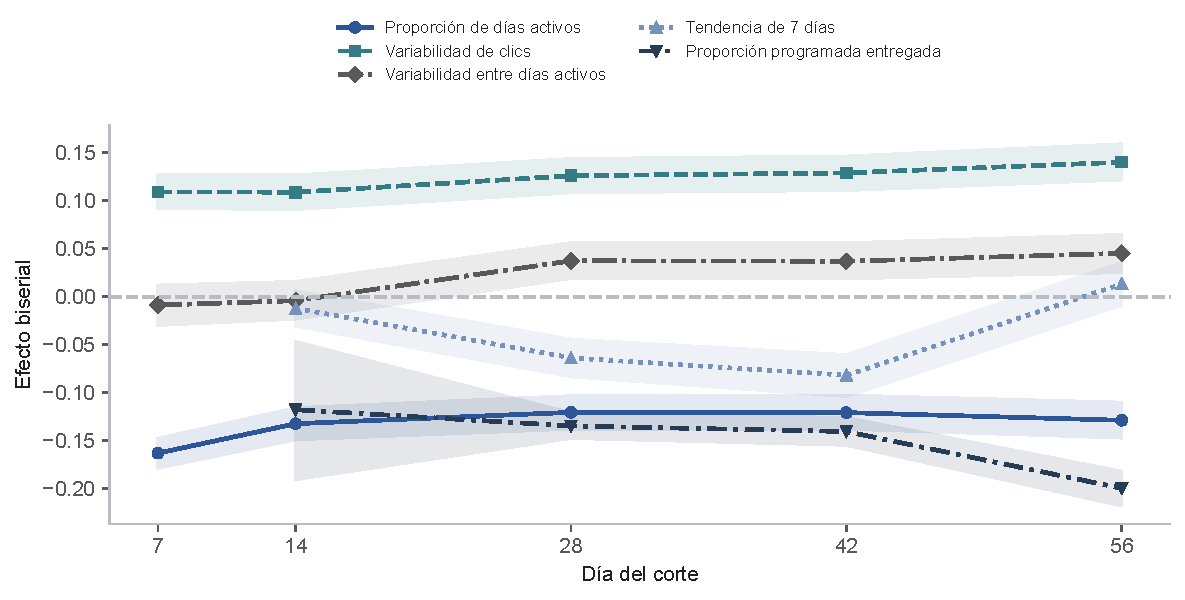
\includegraphics[width=.94\linewidth]{figuras_multiventana/03_efectos_cortes.pdf}
\caption{Efectos por corte e intervalos puntuales mediante remuestreo de personas. Las líneas conectan estimaciones y no representan un contraste longitudinal.}\label{multi03:figefectos}\end{figure}
En la figura, el eje horizontal indica el día de corte y el vertical el efecto estimado. Un valor por debajo de cero señala valores generalmente menores entre las inscripciones con retiro futuro; uno por encima señala valores mayores. Las franjas alrededor de las líneas muestran la incertidumbre de cada estimación.

La tendencia de siete días en el corte 56 presenta un efecto de 0,013, con intervalo de -0,009 a 0,036. Este resultado no respalda una dirección clara de asociación para ese indicador en ese corte; tampoco demuestra ausencia de utilidad predictiva conjunta. La tendencia de catorce días conserva un significado distinto porque resume dos bloques de mayor duración.

\Needspace{.14\textheight}\subsection{Disponibilidad, distribución y heterogeneidad}
Dividir la actividad y la recencia por los días observados facilita comparar ventanas de distinta duración. Sin embargo, esta operación no iguala las oportunidades de participación y evaluación de los cursos. Las distribuciones empíricas se presentan por corte y las tablas completas conservan los tamaños observados y ausentes. La proporción entregada se analiza solo donde hay evaluaciones programadas; en el día 7 no existe este denominador y no se estima un efecto.


Las curvas de la figura son acumuladas: para un valor del eje horizontal, la altura indica la proporción de inscripciones cuyo indicador es menor o igual a ese valor. Por ejemplo, una altura de 0,60 en una proporción de días activos de 0,40 significaría que el 60 por ciento tuvo actividad en, como máximo, el 40 por ciento de los días observados. Este ejemplo ilustra la lectura y no corresponde a una estimación adicional del estudio.

\begin{figure}[htbp]\centering
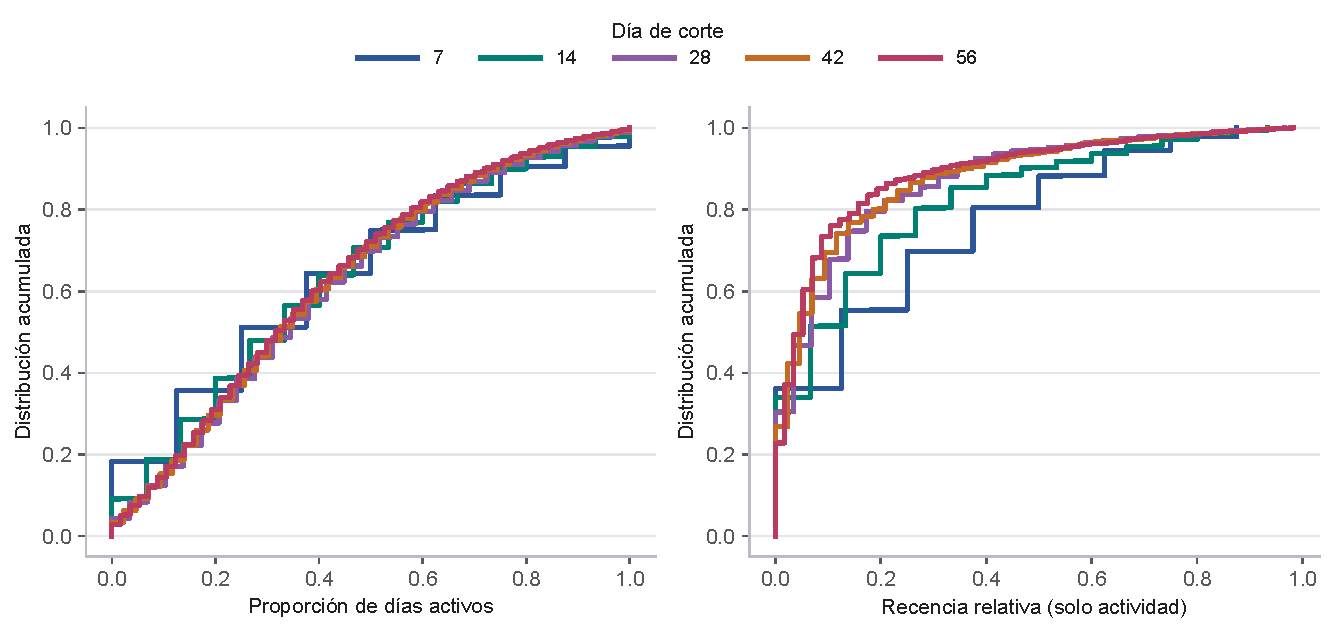
\includegraphics[width=.94\linewidth]{figuras_multiventana/03_distribuciones_cortes.pdf}
\caption{Distribuciones acumuladas de actividad relativa y recencia relativa; esta última excluye inscripciones sin actividad observable.}\label{multi03:distribuciones}\end{figure}

Para variables expresadas en categorías, como el módulo o la región, se utiliza la V de Cramér. Resume cuánto difiere la distribución del retiro entre categorías: valores próximos a cero indican poca asociación descriptiva y valores mayores indican una asociación más marcada. La V de Cramér se calcula como $V_C=\sqrt{\chi^2/[N\min(f-1,g-1)]}$, donde la tabla de contingencia reúne los conteos por categoría y retiro; $N$ es su total, $f$ el número de filas y $g$ el número de columnas. El estadístico $\chi^2$ resume las diferencias entre esos conteos y los que se esperarían si no hubiera asociación. Se utiliza como medida descriptiva de asociación, sin atribuir a su valor significancia estadística ni crecimiento necesario por desbalance de categorías.

\Needspace{.16\textheight}
\begingroup\small\setlength{\tabcolsep}{3pt}\renewcommand{\arraystretch}{1.16}
\begin{longtable}{>{\raggedright\arraybackslash}p{0.29690721649484536\linewidth}>{\raggedright\arraybackslash}p{0.12061855670103093\linewidth}>{\raggedright\arraybackslash}p{0.12061855670103093\linewidth}>{\raggedright\arraybackslash}p{0.12061855670103093\linewidth}>{\raggedright\arraybackslash}p{0.12061855670103093\linewidth}>{\raggedright\arraybackslash}p{0.12061855670103093\linewidth}}
\caption{V de Cramér descriptiva; sin interpretación causal ni pruebas por filas independientes.}\label{multi03:categorias}\\
\toprule
\textbf{Categoría} & \textbf{7} & \textbf{14} & \textbf{28} & \textbf{42} & \textbf{56} \\
\midrule\endfirsthead
\toprule
\textbf{Categoría} & \textbf{7} & \textbf{14} & \textbf{28} & \textbf{42} & \textbf{56} \\
\midrule\endhead
\bottomrule\endfoot
Edad & 0,026 & 0,016 & 0,012 & 0,011 & 0,011 \\*
Módulo & 0,173 & 0,170 & 0,159 & 0,144 & 0,137 \\*
Presentación & 0,082 & 0,059 & 0,043 & 0,040 & 0,033 \\*
Discapacidad & 0,061 & 0,065 & 0,065 & 0,065 & 0,064 \\*
Género & 0,035 & 0,029 & 0,029 & 0,025 & 0,024 \\*
Educación previa & 0,071 & 0,057 & 0,051 & 0,045 & 0,038 \\*
Privación (IMD) & 0,073 & 0,055 & 0,049 & 0,052 & 0,051 \\*
Región & 0,043 & 0,026 & 0,026 & 0,027 & 0,029 \\*
\end{longtable}\endgroup
En la Tabla~\ref{multi03:categorias}, el módulo presenta los mayores valores de V de Cramér entre los atributos publicados en todos los cortes. Esta heterogeneidad contextual debe considerarse al diseñar la validación. La V de Cramér no indica una dirección del efecto ni ajusta por otros atributos. Las tasas por nivel y los conteos se publican en el Anexo~\ref{corr:anexocontexto}, Tabla~\ref{corr:niveles}; que dos categorías tengan porcentajes de retiro distintos no demuestra que pertenecer a una de ellas cause el retiro. Por ejemplo, una diferencia entre módulos puede coincidir con diferencias de calendario, evaluaciones o composición de estudiantes que esta comparación aislada no separa.

La Figura~\ref{fig:contexto-asociaciones} complementa la Tabla~\ref{multi03:categorias}: el color permite reconocer que el módulo presenta la asociación descriptiva más marcada entre las variables comparadas. Cada celda conserva el valor numérico para facilitar su consulta. La escala mostrada termina en 0,20 para distinguir los valores observados; la medida V de Cramér está definida entre cero y uno, y no expresa por sí misma dirección ni causalidad.
\begin{figure}[H]\centering
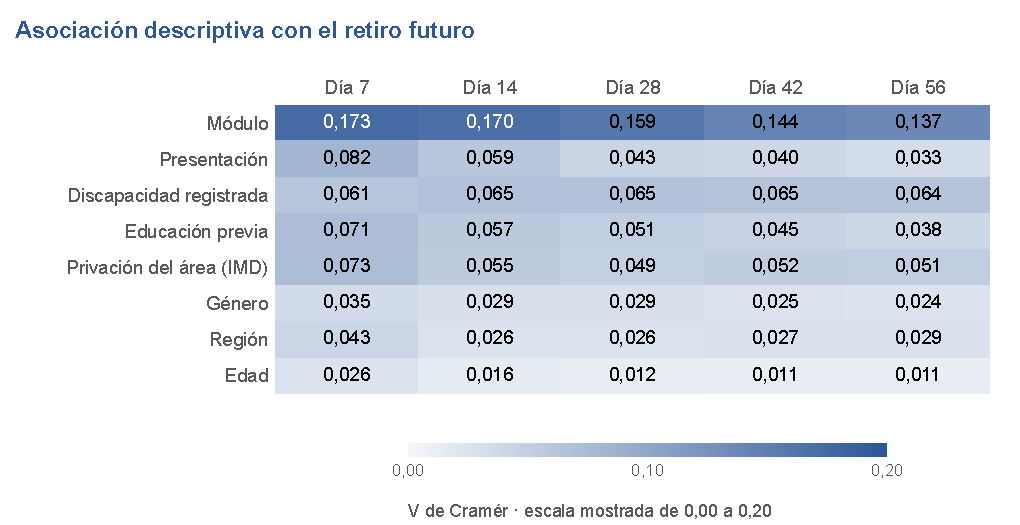
\includegraphics[width=\linewidth]{figuras_contexto/asociaciones_contexto.pdf}
\caption[Asociación descriptiva entre variables de contexto y retiro futuro.]{Asociación descriptiva entre variables de contexto y retiro futuro en cada corte. Elaboración propia a partir de la Tabla~\ref{multi03:categorias}; los tonos oscuros indican valores mayores de V de Cramér.}\label{fig:contexto-asociaciones}
\end{figure}

\Needspace{.16\textheight}\section{Resultados ampliados de las variables de contexto}
Las categorías se analizan en las mismas poblaciones de cada corte. La Tabla~\ref{corr:niveles} publica conteos y tasas por nivel; la categoría No disponible identifica los casos sin dato de IMD. Este índice describe la privación socioeconómica del área de residencia; no mide directamente los ingresos de la persona \cite{sdata2017171}. Mantener esos casos identificados permite mostrar cuántos carecen de esa información, sin asignarles una categoría socioeconómica supuesta. Esta comparación muestra asociaciones observadas, pero no separa todas las características que pueden influir conjuntamente. Tampoco permite concluir si un modelo trata de forma equitativa a distintos grupos: todavía no se han evaluado sus predicciones y errores por grupo.

% Figuras reproducibles: scripts/figuras_cuerpo.py. Las tablas del anexo se conservan.
Las Figuras~\ref{fig:contexto-edad} a~\ref{fig:contexto-region} presentan el corte 28 como ejemplo de lectura de las categorías; esta elección no establece que sea el mejor momento para predecir. En ese corte se incluyen 27\,515 inscripciones elegibles y se observan 5\,012 retiros posteriores, equivalentes al 18,2\%. Cada barra expresa el porcentaje dentro de su categoría y la línea discontinua señala el porcentaje general. Los conteos completos de los cinco cortes permanecen en el Anexo~\ref{corr:anexocontexto}, Tabla~\ref{corr:niveles}.

\Needspace{.40\textheight}\subsection{Edad y discapacidad registrada}
La Figura~\ref{fig:contexto-edad} permite comparar los porcentajes de retiro sin perder de vista el tamaño de cada grupo. La categoría de 55 o más años reúne solo 193 inscripciones, frente a 19\,166 en la primera banda. Por ello, los porcentajes deben leerse junto con sus denominadores; el menor porcentaje observado en un grupo pequeño no demuestra una ventaja general asociada con la edad. Se conservan las bandas definidas por OULAD.
\begin{figure}[H]\centering
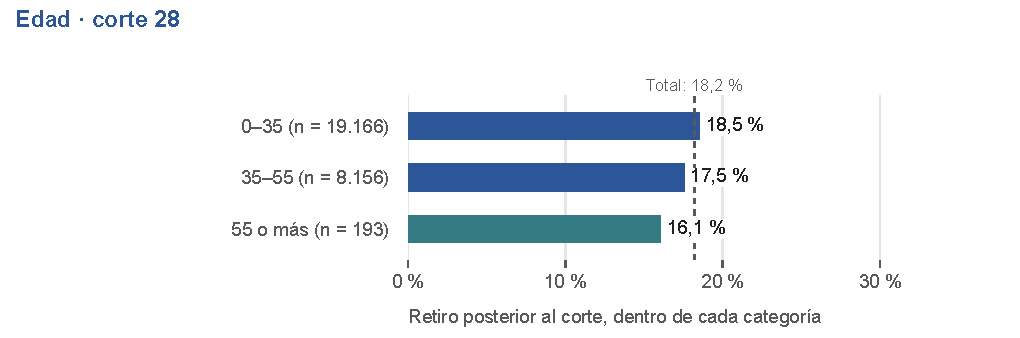
\includegraphics[width=\linewidth]{figuras_contexto/contexto_age_band_28.pdf}
\caption[Retiro futuro por banda de edad al día 28.]{Retiro futuro por banda de edad al día 28. $n$ indica inscripciones de cada categoría. Elaboración propia a partir de los conteos de la Tabla~\ref{corr:niveles} del anexo.}\label{fig:contexto-edad}
\end{figure}

La Figura~\ref{fig:contexto-discapacidad} muestra un porcentaje observado de 26,0\% entre las inscripciones con discapacidad registrada y de 17,4\% entre aquellas sin ese registro afirmativo. La diferencia descriptiva es de 8,6 puntos porcentuales. Esta comparación no ajusta por módulo, calendario u otras características y no identifica la causa de la diferencia.
\begin{figure}[H]\centering
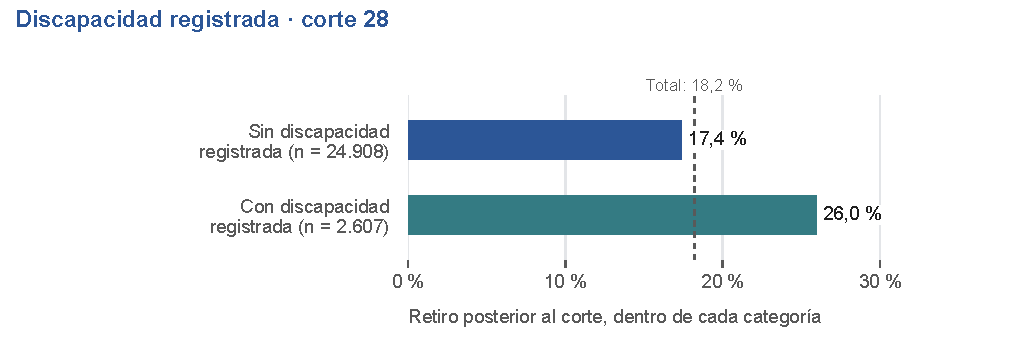
\includegraphics[width=\linewidth]{figuras_contexto/contexto_disability_28.pdf}
\caption[Retiro futuro según discapacidad registrada al día 28.]{Retiro futuro según discapacidad registrada al día 28. Los tamaños de los grupos se muestran junto a las etiquetas. Elaboración propia; conteos en la Tabla~\ref{corr:niveles} del anexo.}\label{fig:contexto-discapacidad}
\end{figure}

\subsection{Privación del área de residencia y región}
Las bandas de IMD se mantienen en su orden original en la Figura~\ref{fig:contexto-imd}. Los porcentajes oscilan entre bandas y no siguen una disminución uniforme. Los casos sin dato se muestran en gris: corresponden a 1\,027 inscripciones y no deben interpretarse como una banda adicional de privación. La figura describe diferencias entre grupos de áreas de residencia, sin trasladar automáticamente esa interpretación a los recursos económicos de cada persona.
\begin{figure}[H]\centering
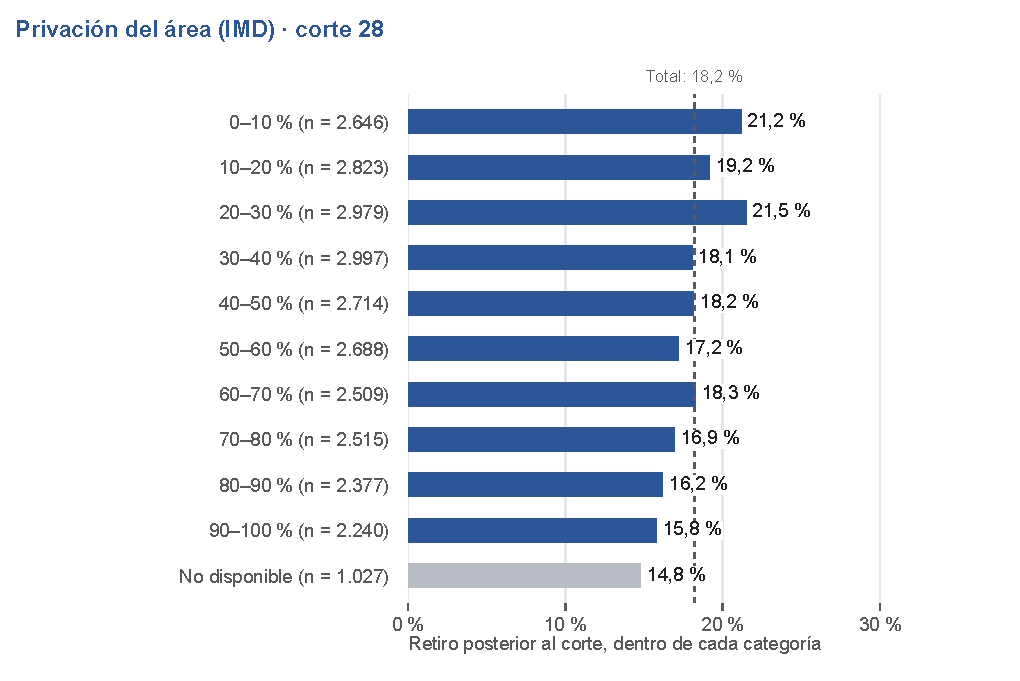
\includegraphics[width=\linewidth]{figuras_contexto/contexto_imd_band_28.pdf}
\caption[Retiro futuro por banda de IMD al día 28.]{Retiro futuro por banda de IMD al día 28. La línea discontinua representa el porcentaje general del corte. Elaboración propia; valores y denominadores en la Tabla~\ref{corr:niveles} del anexo.}\label{fig:contexto-imd}
\end{figure}

En la Figura~\ref{fig:contexto-region}, las regiones se ordenan por su porcentaje observado para facilitar la comparación. El rango va de 16,7\% en East Anglian Region a 19,8\% en West Midlands Region. Este orden resume el corte 28 y no constituye una clasificación permanente de las regiones ni una comparación ajustada de sus condiciones educativas.
\begin{figure}[H]\centering
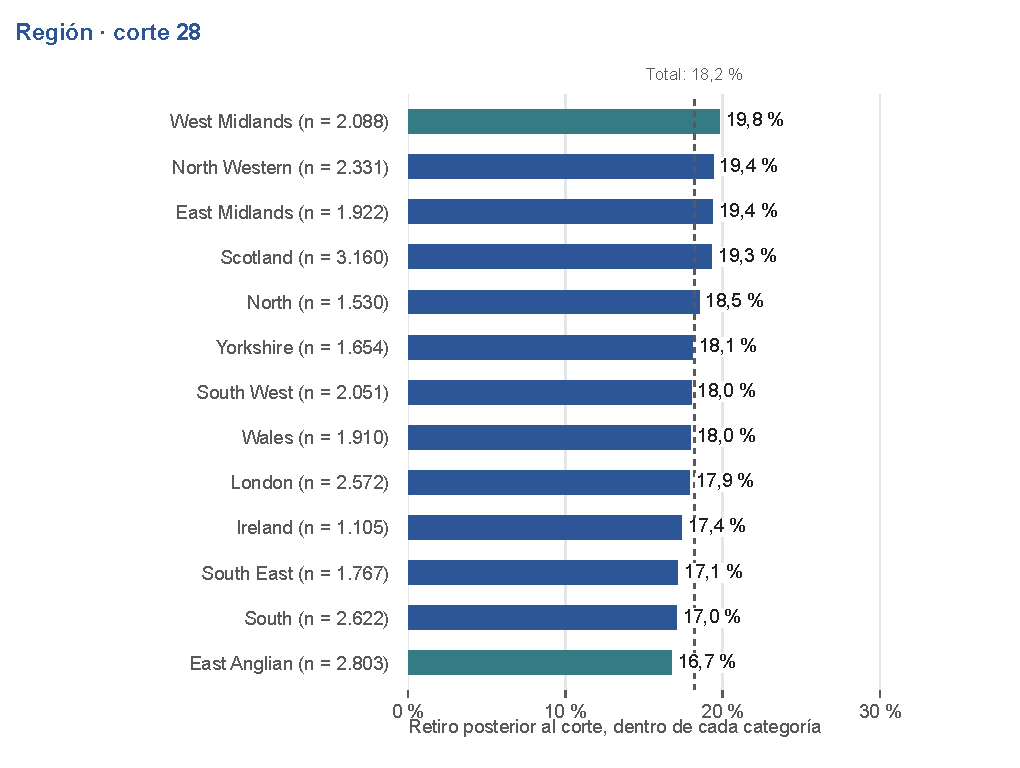
\includegraphics[width=\linewidth]{figuras_contexto/contexto_region_28.pdf}
\caption[Retiro futuro por región al día 28.]{Retiro futuro por región al día 28. Se abrevia la palabra \textit{Region} en las etiquetas. Elaboración propia; conteos completos en la Tabla~\ref{corr:niveles} del anexo.}\label{fig:contexto-region}
\end{figure}

\subsection{Lectura conjunta de los cinco cortes}
Las Figuras~\ref{fig:contexto-cortes} y~\ref{fig:contexto-region-cortes} reúnen los porcentajes de los cinco cortes mediante una escala común: un azul más oscuro representa un porcentaje mayor. Cada columna identifica su población elegible. La lectura horizontal describe cómo cambian los porcentajes publicados, pero no sigue una población fija: entre cortes cambian las inscripciones incluidas y el tiempo restante hasta el final del curso. Por ello, una reducción del porcentaje no demuestra una mejora predictiva ni una disminución del riesgo de una misma persona.
\begin{figure}[H]\centering
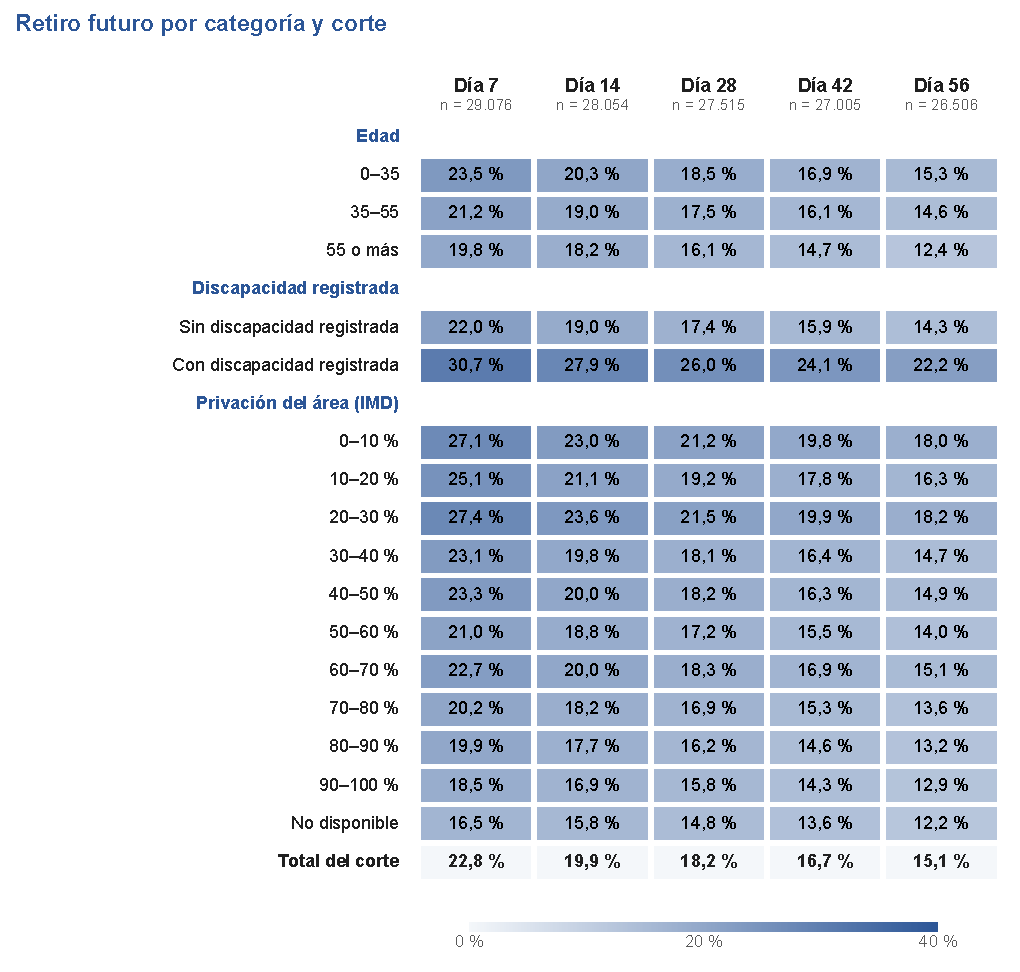
\includegraphics[width=\linewidth]{figuras_contexto/contexto_cortes.pdf}
\caption[Retiro futuro por edad, discapacidad e IMD en cinco cortes.]{Retiro futuro por edad, discapacidad registrada e IMD en los cinco cortes. La fila final muestra el porcentaje general de cada corte. Elaboración propia; numeradores y denominadores por categoría en la Tabla~\ref{corr:niveles} del anexo.}\label{fig:contexto-cortes}
\end{figure}

La Figura~\ref{fig:contexto-region-cortes} conserva el mismo orden alfabético de las regiones en todas las columnas. Esta disposición permite localizar cada región sin confundir un cambio en el orden de las filas con un cambio en los resultados. Los valores corresponden al retiro registrado después de cada corte y hasta el final del curso.
\begin{figure}[H]\centering
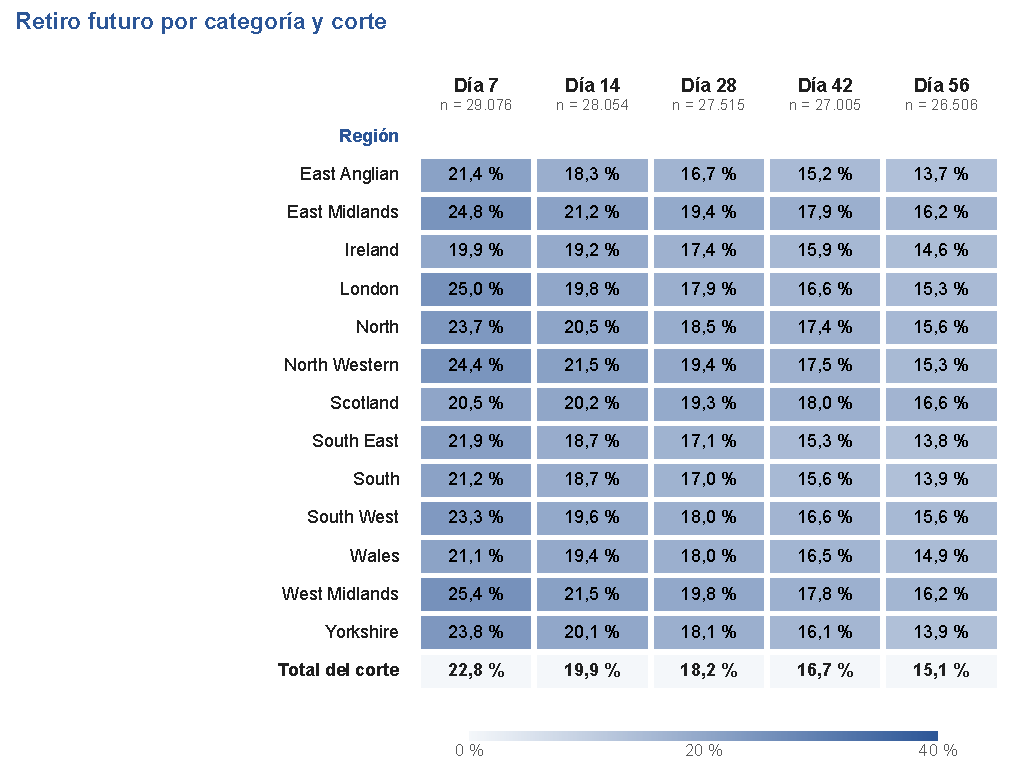
\includegraphics[width=\linewidth]{figuras_contexto/contexto_region_cortes.pdf}
\caption[Retiro futuro por región en cinco cortes.]{Retiro futuro por región en los cinco cortes. Se utiliza la misma escala de color que en la Figura~\ref{fig:contexto-cortes}. Elaboración propia; detalle en la Tabla~\ref{corr:niveles} del anexo.}\label{fig:contexto-region-cortes}
\end{figure}

\Needspace{.42\textheight}\subsection{Créditos e intentos previos}

\Needspace{.16\textheight}
\begingroup\small\setlength{\tabcolsep}{3pt}\renewcommand{\arraystretch}{1.16}
\begin{longtable}{>{\raggedright\arraybackslash}p{0.0782608695652174\linewidth}>{\raggedright\arraybackslash}p{0.1858695652173913\linewidth}>{\raggedright\arraybackslash}p{0.13695652173913045\linewidth}>{\raggedright\arraybackslash}p{0.11739130434782608\linewidth}>{\raggedright\arraybackslash}p{0.11739130434782608\linewidth}>{\raggedright\arraybackslash}p{0.14673913043478262\linewidth}>{\raggedright\arraybackslash}p{0.11739130434782608\linewidth}}
\caption{Distribución y asociación de créditos e intentos previos; efecto biserial por rangos.}\label{corr:numericos}\\
\toprule
\textbf{Corte} & \textbf{Variable} & \textbf{Observados} & \textbf{Ausentes} & \textbf{Mediana} & \textbf{Q25--Q75} & \textbf{Efecto} \\
\midrule\endfirsthead
\toprule
\textbf{Corte} & \textbf{Variable} & \textbf{Observados} & \textbf{Ausentes} & \textbf{Mediana} & \textbf{Q25--Q75} & \textbf{Efecto} \\
\midrule\endhead
\bottomrule\endfoot
7 & Créditos & 29\,076 & 0 & 60,000 & 60--90 & 0,165 \\*
7 & Intentos previos & 29\,076 & 0 & 0,000 & 0--0 & 0,028 \\*
14 & Créditos & 28\,054 & 0 & 60,000 & 60--90 & 0,138 \\*
14 & Intentos previos & 28\,054 & 0 & 0,000 & 0--0 & 0,030 \\*
28 & Créditos & 27\,515 & 0 & 60,000 & 60--90 & 0,131 \\*
28 & Intentos previos & 27\,515 & 0 & 0,000 & 0--0 & 0,033 \\*
42 & Créditos & 27\,005 & 0 & 60,000 & 60--90 & 0,125 \\*
42 & Intentos previos & 27\,005 & 0 & 0,000 & 0--0 & 0,036 \\*
56 & Créditos & 26\,506 & 0 & 60,000 & 60--90 & 0,119 \\*
56 & Intentos previos & 26\,506 & 0 & 0,000 & 0--0 & 0,038 \\*
\end{longtable}\endgroup
Los créditos indican el total registrado para los módulos que cursa la persona, mientras que los intentos previos cuentan cuántas veces había intentado cursar ese módulo \cite{sdata2017171}. En la tabla, la mediana es el valor central y Q25--Q75 delimita la mitad central de los datos. Por ejemplo, 60--90 significa que esa mitad se sitúa entre 60 y 90 créditos; no es el intervalo de incertidumbre de la asociación. En particular, la fila de créditos del corte 56 resume 26\,506 inscripciones con información disponible, mediana de 60 créditos y efecto de 0,119. Este último valor señala que los créditos tienden a ser mayores entre las inscripciones con retiro futuro; no significa que aumentar la carga cause el retiro ni que reducirla evite ese resultado. Los créditos y los intentos previos se conservan como información de contexto y no se incorporan automáticamente a los indicadores de actividad.
Los conteos por nivel se publican en el Anexo~\ref{corr:anexocontexto}, Tabla~\ref{corr:niveles}.

\Needspace{.10\textheight}\section{Síntesis de la caracterización}
La revisión precisó que cada fila de la base integrada representa una inscripción y permitió distinguir el retiro administrativo de la inactividad. Las asociaciones observadas orientan la preparación de los datos, pero aún no muestran cómo funcionará un modelo con casos nuevos.

El capítulo siguiente explica quiénes se incluyen en cada corte y cómo se construyen sus indicadores, conservando la distinción entre ausencia de actividad e información que no puede calcularse.
